
\subsection{State}
\begin{frame}{\textbf{State}}
    The state is the place where the program stores its variables and data.
    \begin{block}{State}
        The state is divided up into two parts:
        \begin{itemize}
            \item \textbf{Enviroment}: The place where the program stores its variables.
                                        dictionary, where keys are variable names and values, are pointers to locations in the store. 
                                        The environment also contains the Free Pointer, which points to the next free location in memory.
            \item \textbf{Store}: The place where the program stores its data, aka Memory.
                                    The store is usually an array of values. Most often the values are bytes and types often take up multiple slots.
                                    Semantic analysis is used to determine the size of the types and to figure out addresses.
        \end{itemize}
    \end{block}
\end{frame}

\subsection{Scoping}
\begin{frame}{\textbf{Scoping}}
    Scoping is the process of determining where a variable is visible to the program.\\
    Scoping is usually divided into three different classes:
    \begin{itemize}
        \item \textbf{Runtime Scoping}
        \item \textbf{Static Scoping}
        \item \textbf{Dynamic Scoping}
    \end{itemize}
\end{frame}

\subsection*{Scoping}
\begin{frame}[fragile]{\textbf{Scoping}}
    \begin{example}
        \lstinputlisting[language=c,basicstyle=\ttfamily\tiny]{examples/scoping/scoping.c}
    \end{example}
\end{frame}



\subsection{Arrays}
\begin{frame}{\textbf{Arrays}}
    \begin{block}{Arrays}
        Arrays are a collection of elements of the same type.
        They're most often stored as a contiguous block of memory.\\
        Formula for accessing an element in an array:
        \begin{equation*}
            \texttt{foo[n]} = \texttt{\&foo} + n * \texttt{sizeof(T)}
        \end{equation*}
        \begin{itemize}
            \item \texttt{\&foo} is the pointer to the array
            \item \texttt{n} is the index of the element we want to access
            \item \texttt{sizeof(T)} is the size of type T in bytes
        \end{itemize}
    \end{block}    
\end{frame}

\subsection*{Arrays}
\begin{frame}[fragile]{\textbf{Arrays}}
    \begin{example}
        \begin{lstlisting}[language=c]
    int foo[5] = {1,2,3,4,5};
        \end{lstlisting}
    \end{example}
\end{frame}

%\begin{frame}{Arrays}
%    \begin{example}
%        \begin{figure}
%            \centering
%            \adjustbox{scale=0.4}{
%                \begin{bytefield}{8}
%                    \begin{rightwordgroup}{\texttt{foo} is a pointer to the array at \texttt{0x00}}
%                        \memsection{0xff}{}{1}{\texttt{foo}}
%                    \end{rightwordgroup}\\
%                    \memsection{0xfe}{}{4}{...}\\
%                    \begin{rightwordgroup}{The actual array}
%                        \memsection{0x13}{}{4}{5}\\
%                        \memsection{0x0f}{}{4}{4}\\
%                        \memsection{0xb}{}{4}{3}\\
%                        \memsection{0x08}{}{4}{2}\\
%                        \memsection{0x04}{0x00}{4}{1}
%                    \end{rightwordgroup}
%                \end{bytefield}
%            }
%        \end{figure}
%    \end{example}
%\end{frame}

\begin{frame}{\textbf{Multidimensional Arrays}}
    Multidimensional arrays are arrays of arrays.
    \begin{block}{Multidimensional Arrays}
        There are two main ways of storing multidimensional arrays:
        \begin{itemize}
            \item \textbf{Array of Pointers}: Each element in the array is a pointer to another array somewhere else in memory.
            \item \textbf{Contiguous Block}: The entire multidimensional array is stored as a contiguous block of memory. Where each row is stored sequentially.
        \end{itemize}
    \end{block}
\end{frame}

\begin{frame}{\textbf{Multidimensional Arrays}}
    \begin{block}{Forumla for Contiguous Block}
        \begin{equation*}
            \texttt{bar[i][j]} = \texttt{\&bar} + i * \texttt{length(row)} + j * \texttt{sizeof(T)}
        \end{equation*}
        where 
        \begin{itemize}
            \item \texttt{\&bar} is the pointer to the array
            \item \texttt{i} is the row index
            \item \texttt{j} is the column index
            \item \texttt{sizeof(T)} is the size of type T in bytes
            \item \texttt{length(row)} is the length of the row
        \end{itemize}
    \end{block}
\end{frame}

\begin{frame}[fragile]{\textbf{Multidimensional Arrays}}
    \begin{example}
        \begin{lstlisting}[language=c]
    int bar[][] = {
            {1,2},
            {3,4}
        };
        \end{lstlisting}
    \end{example}
\end{frame}

\subsection{Records}
\begin{frame}{\textbf{Records}}
    Records are a collection of elements of different types.
    Each element is called a field.\\
    \begin{block}{Records}
        Records are stored as a contiguous block of memory. With each field stored consecutively.\\
        To access a field in a record we need to know the offset of the field in the record.
    \end{block}
\end{frame}

\subsection*{Records}
\begin{frame}{\textbf{Records}}
    \begin{block}{Records}
        Formula for accessing a field in a record:
        \begin{equation*}
            \texttt{foo.bar} = \texttt{\&foo} + \texttt{offset(bar)}
        \end{equation*}
        where 
        \begin{itemize}
            \item \texttt{\&foo} is the pointer to the record
            \item \texttt{bar} is the field that we want to access
            \item \texttt{offset(bar)} is the offset of the field \texttt{bar} in the record
        \end{itemize}
    \end{block}
\end{frame}

\begin{frame}[fragile]{\textbf{Records}}
    \begin{example}
        \begin{lstlisting}[language=c]
    struct foo {
        int x; //Offset 0
        bool y; //Offset 4
        double z; //Offset 5
    };
        \end{lstlisting}
    \end{example}
\end{frame}

\begin{frame}{\textbf{Arrays of Records}}
    \begin{block}{Records}
        Formula for accessing a field of the nth element in an array of records:
        \begin{equation}
            \texttt{foo[n].bar} = \texttt{\&foo} + n * \texttt{sizeof(T)} + \texttt{offset(bar)}
        \end{equation}
        where 
        \begin{itemize}
            \item \texttt{\&foo} is the pointer to the array
            \item \texttt{n} is the index of the element we want to access
            \item \texttt{sizeof(T)} is the size of type T in bytes
            \item \texttt{bar} is the field that we want to access
            \item \texttt{offset(bar)} is the offset of the field \texttt{bar} in the record
        \end{itemize}
    \end{block}
\end{frame}

\subsection*{Q\&A}
\begin{frame}{Questions?}
    \begin{figure}
        \centering
        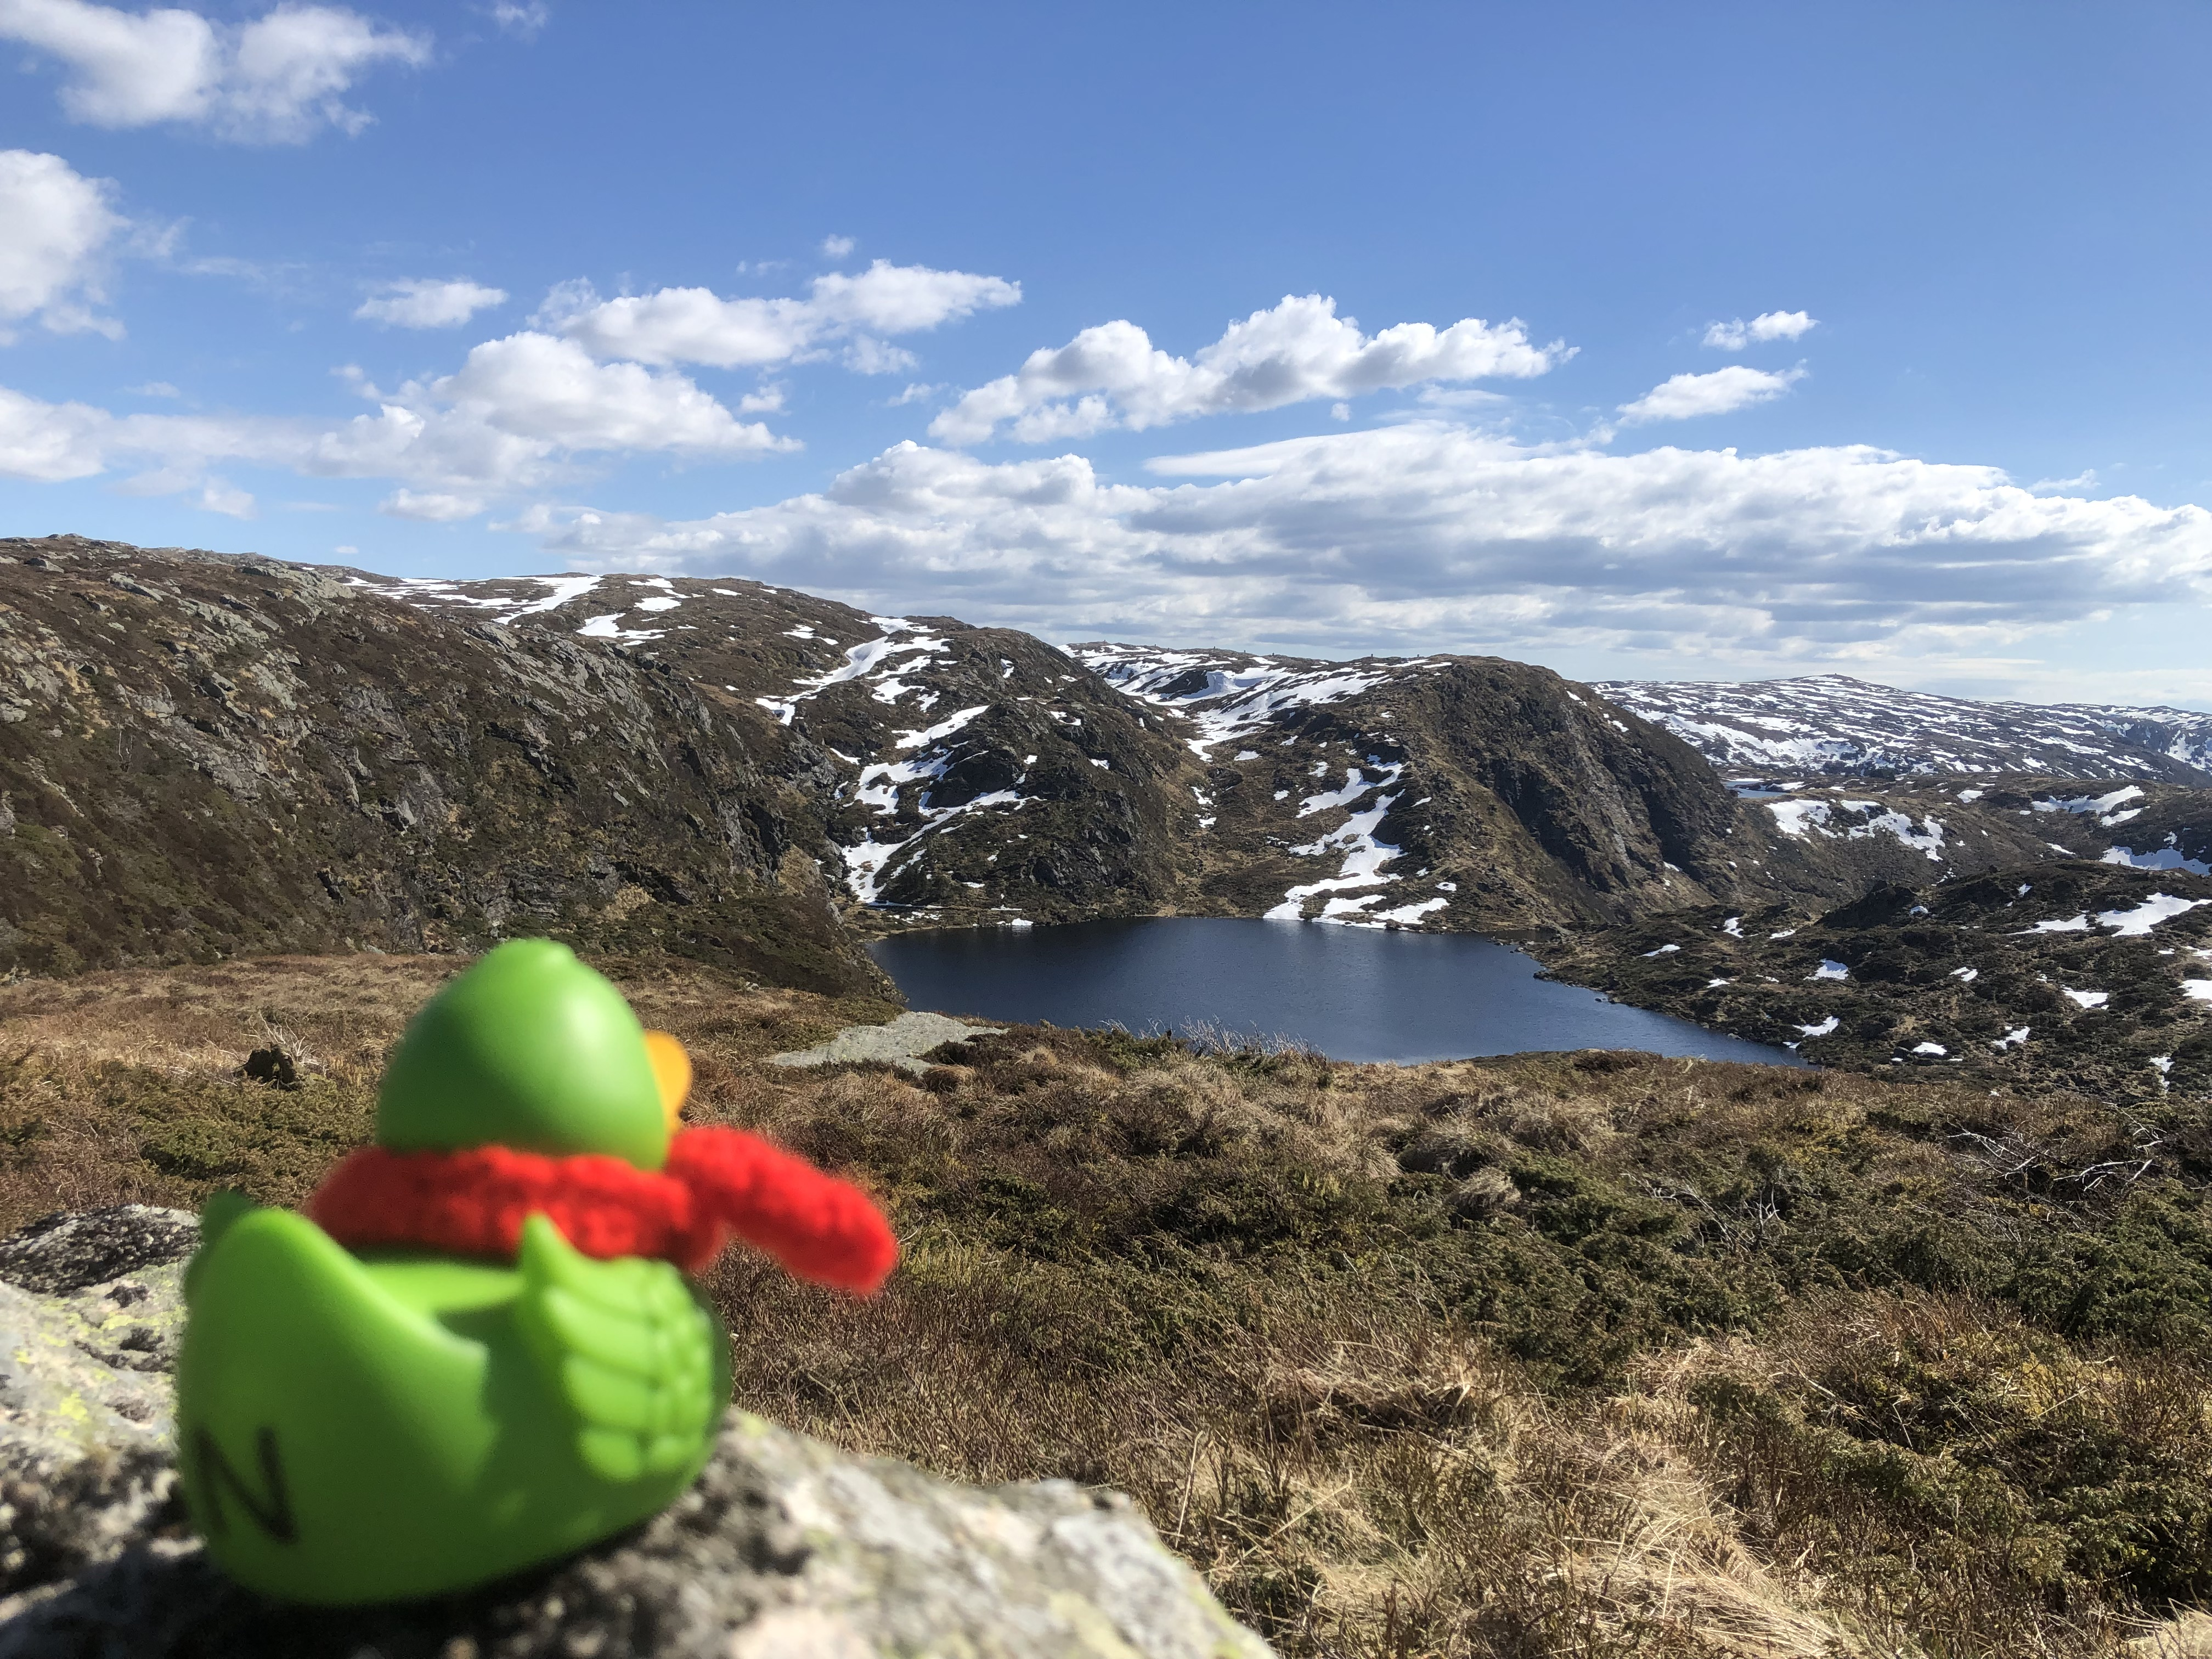
\includegraphics[height = 4.9cm]{guillaume4.jpg}
    \end{figure}
\end{frame}